\begin{example} \label{eg:6.3.1} % EXAMPLE
Find the arc length of $f(x) = x^{3/2}$ from $x=0$ to $x=4$. 

\solution
We begin by finding $\fp(x)= \frac32x^{1/2}$. Using the formula, we find the arc length $L$ as
\begin{align*}
	L &=	\int_0^4 \sqrt{1+\left(\frac32x^{1/2}\right)^2}\ dx \\
		&=	\int_0^4 \sqrt{1+\frac94x} \ dx \\
		&= 	\int_0^4 \left(1+\frac94x\right)^{1/2}\ dx \\
		&=  \frac23\frac49\left(1+\frac94x\right)^{3/2}\Big|_0^4 \\
		&=\frac{8}{27}\left(10^{3/2}-1\right) \approx 9.07 \text{units}.
\end{align*}
A graph of $f$ is given in Figure \ref{F:6.3.Ex1}.
\end{example}

\begin{marginfigure}[-8cm] %MARGIN FIGURE
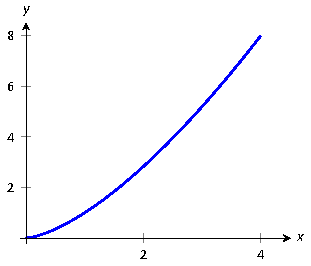
\includegraphics{figures/figarc1}
\caption{A graph of $f(x) = x^{3/2}$ from Example~\ref{eg:6.3.1}.} \label{F:6.3.Ex1}
\end{marginfigure}

